The models that used the Window declustering catalogue have in the word Window appended at their names or SLC, for the methods that used the Single Link Cluster. 


\section{Experimental Design}
The first experiment was made to compare the all the models proposed with each other and to discover which method would achieve higher log-likelihood values. We created some scenarios (space/time regions), and we applied the methods for for the regions of Kanto, Kansai, Touhoku and East Japan for a given year (2005-2010) with earthquakes with depth lesser than 100km. We also used 3 kinds of catalogues with the minimum magnitude of 3.0: the JMA and the declustered catalogues form the Window method and the SLC method. 

We compared the means of the models log-likelihood values using the ANOVA test. If a group of variables considered for the ANOVA test showed no statistically significant difference, we applied the Paired Student t-test, in the case all groups showed statistically significant difference, the Tukey HSD methodology analysis was used.

The second experiment was made a to compare how the magnitude of the earthquakes influence the models generated. We used the same scenarios from the first experiment. We split the models obtained from these scenarios into slices composed of earthquakes that have magnitude in a given magnitude interval. We calculated the log-likelihood of these slices-models and applied the ANOVA test and the Tukey HSD to compared them.


\subsection{Details of the Statistical Analysis}\label{anova}
The goal is to discover if there is any variation between the methods and which are the most influential variables. To achieve that, we used the ANOVA test, because it indicates that the means of several groups are equal or not for a given confidence interval. The confidence interval was set to 95\%, meaning that if the ``p-value'' is smaller than 0.05 it signifies that there exists a statistical significant evidence that the variables variance are different from each other.

The hypothesis for this experiment can be generalised as follows:

$$\begin{cases} H_0: \text{The population means are equal.} &\\
H_1: \text{The population means are different.}&\\
\end{cases}$$\\

The Tukey HSD is applied on the results obtained from the ANOVA test to specify which groups differ, in the case any group has a ``p-value'' lesser than 0.05. Tukey's methodology analysis shows the means of a case with the means of every other case. Doing so, it identifies differences between means :

$$\begin{cases}
\mu_a-\mu_b, \text{where $\mu_a$ is the mean of the first group}\\
                \text{$\mu_b$ is the mean of the second group.}
\end{cases}$$

In the case where statistical significant difference exists, we explore this by pairing the measures observations of two groups. That is:

$$\begin{cases}
H_0: \mu = 0, \text{the difference between observations is 0.}&\\
H_1: \mu != 0, \text{difference between observations is not 0.}
\end{cases}$$\\


\subsection{Results from The Mainshock Models Mainshock with Aftershock Models Experiment}\label{resultsBigExp}

An one-way between subjects ANOVA was conducted to compare the effects of the models, the years and regions on the log-likelihood value. The models compared are: ReducedGAModel, Emp-ReducedGAModelSLC, Emp-GAModel, Emp-ReducedGAModel, GAModelWindow, ReducedGAModelWindow, GAModelSLC, ReducedGAModelSLC, Emp-GAModelWindow, Emp-ReducedGAModelWindow, GAModel and Emp-GAModelSLC.

Based on the results of the ANOVA test, it is evident that all variables are significantly different. The results of the experiments are in the Table~\ref{anovatest1}. All variables had a ``p-value'' lower than 0.05, indicating that they can be considered different.

%TODO: pegar monografia e ver o que eu tinha pensado
\begin{table*}[]
	\centering
	\begin{tabular}{|l|l|l|l|l|l|}
		\hline
		{Variable} & {Degrees of Freedom} & {Sum Sq}    & {Mean Sq}   & {F Value} & {Pr(\textgreater F)} \\
		\hline
		Model    & 15           	  & 149303768  & 9953585   & 63.72    & \textless2e-16     \\
		\hline
		Year     & 5                  & 414016420  & 82803284  & 530.06   & \textless2e-16     \\
		\hline
		Region   & 3                  & 869821655  & 289940552  & 1856.02   & \textless2e-16	\\    
		\hline
	\end{tabular}
	\caption{ANOVA Test Results Values - Mainshock Models Mainshock and Aftershock Models.}
	\label{anovatest1}
\end{table*}

Because we found statistically significant result, we applied a Post-hoc comparisons using the Tukey HSD analysis methodology on the ANOVA result. It compared each condition with all others. For example, it compares the values from the GAModel with the GAModelWindow. 

It indicated that the models GAModelSLC, Emp-ReducedGAModelWindow, GAModelWindow, ReducedGAModelWindow, ReducedGAModelSLC achieve statistically better or equal results in terms of log-likelihood when compared with the other models. When they are compared with themselves, they are statistically equal. 

We applied the ANOVA test now only with this 5 models. The models group have a ``p-value'' of 0.171, indicating that they have similar log-likelihood values. The results are in the Table~\ref{anovatest2}.
     
\begin{table*}[]
	\centering
	\begin{tabular}{|l|l|l|l|l|l|}
		\hline
		{Variable} & {Degrees of Freedom} & {Sum Sq}    & {Mean Sq}   & {F Value} & {Pr(\textgreater F)} \\
		\hline
		Model    & 4           	  & 884882  & 221220   & 1.604    & 0.171    \\
		\hline
		Year     & 5                 & 150297410  & 30059482  & 217.955   & \textless2e-16     \\
		\hline
		Region   & 3                  & 234225270  & 78075090  & 566.107   & \textless2e-16	\\    
		\hline
	\end{tabular}
	\caption{ANOVA Test Results Values - Emp-ReducedGAModelWindow, GAModelWindow, ReducedGAModelWindow, GAModelSLC, ReducedGAModelSLC.}
	\label{anovatest2}
\end{table*}

Therefore, to confirm that the models are statistically equal, we conducted the Tukey HSD on this ANOVA result. This time, we found statistically significant difference only for the year and region groups. To show that the models results are not statistically different from each other, we applied a pairing analysis.

From the the pairing analysis, we decided to use the \textit{ReducedGAModelSLC} as the representative method of this study. That is because, in all cases when its values were compared, it showed a better performance in the means of the log-likelihood values and in only one case the ``p-value'' was higher than 0.05. For the results, see the Table~\ref{Paired}.

%In this Table, the column labelled $\mu_a - \mu_b$ shows the result of paired difference between the models referred in the ``Models Compared'' column. The ``p-value'' shows the significance value of the paired {\it Student's t-test} for the null hypothesis ``The paired difference of the means of the models is equal''.


\begin{table*}[]
	\begin{center}
		\begin{tabular}{|c|c|c|c|}
			\hline
			\multicolumn{1}{|c|}{Region} &
			\multicolumn{1}{|c|}{Models Compared} & \multicolumn{1}{|c|}{Mean of $\mu_a - \mu_b$}&
			\multicolumn{1}{|c|}{p-value} \\
			\hline
			
			Kansai & \textbf{EMP-GAModelWindow} - GAModelWindow &
			 38.67553 &  3.304e-05 \\
			
		    & \textbf{EMP-GAModelWindow} - ReducedGAModelWindow & 4.272185  & 0.2607\\
			
			& \textbf{EMP-GAModelWindow} - GAModelSLC & 
			112.0424 &  1.122e-05\\

			&EMP-GAModelWindow - \underline{\textbf{ReducedGAModelSLC}} &  
			-1.787262 & 0.5673 \\
			
			& GAModelWindow - \textbf{ReducedGAModelWindow} &
			-34.40335 & 0.000963\\
			
			& \textbf{GAModelWindow} - GAModelSLC &
			 73.36687  &9.065e-06\\
				
			& GAModelWindow - \underline{\textbf{ReducedGAModelSLC}} &
			-40.46279 & 6.32e-05\\
				
			& \textbf{ReducedGAModelWindow} - GAModelSLC &
			107.7702  & 2.632e-05\\

			& ReducedGAModelWindow - \underline{\textbf{ReducedGAModelSLC}} &
			-6.059447 &0.2982\\

			& GAModelSLC - \underline{\textbf{ReducedGAModelSLC}} &
			-113.8297 & 1.2e-05\\

			\hline
			Touhoku & EMP-\textbf{GAModelWindow} - GAModelWindow &
			3.34556 & 0.546\\
			& \textbf{EMP-GAModelWindow} - ReducedGAModelWindow &
			81.60965 & 5.225e-07\\
			&	\textbf{EMP-GAModelWindow} - GAModelSLC &
			63.02216 &0.01971\\
			& EMP-GAModelWindow - \underline{\textbf{ReducedGAModelSLC}} &
			-62.70586 & 0.007075\\
			& \textbf{GAModelWindow} - ReducedGAModelWindow & 
			78.26409 & 2.938e-05\\
			& \textbf{GAModelWindow} - GAModelSLC &
			59.6766 & 0.04829\\
			& GAModelWindow - \underline{\textbf{ReducedGAModelSLC}} &
			-66.05142 &0.001231\\
			& ReducedGAModelWindow - \textbf{GAModelSLC} &
			-18.58749 & 0.3443\\
			& ReducedGAModelWindow - \underline{\textbf{ReducedGAModelSLC}} &
			-144.3155 & 0.000214\\
			& GAModelSLC - \underline{\textbf{ReducedGAModelSLC}} &
			-125.728 &0.01216\\

			
			\hline
			East Japan & \textbf{EMP-GAModelWindow} - GAModelWindow &
			1.872764  & 0.9539\\

			& \textbf{EMP-GAModelWindow} - ReducedGAModelWindow &
			194.4944 & 1.834e-06\\
			& \textbf{EMP-GAModelWindow} - GAModelSLC &
			189.1155 & 0.0003456\\
			& EMP-GAModelWindow - \underline{\textbf{ReducedGAModelSLC}} &
			-274.9858 & 4.961e-05\\
			& \textbf{GAModelWindow} - ReducedGAModelWindow &
			192.6217 & 0.003738\\
			& \textbf{GAModelWindow} - GAModelSLC &
			187.2428 &9.495e-06\\
			& GAModelWindow - \underline{\textbf{ReducedGAModelSLC}} &
			-276.8586 & 4.636e-05\\
			& ReducedGAModelWindow - \textbf{GAModelSLC} & 
			-5.378912 & 0.8576\\
			& ReducedGAModelWindow - \underline{\textbf{ReducedGAModelSLC}} &
			-469.4803 & 1.446e-05\\
			& GAModelSLC - \underline{\textbf{ReducedGAModelSLC}} &
			-464.1014  & 2.38e-06\\

			
			\hline
			Kanto & EMP-\textbf{GAModelWindow} - GAModelWindow &
			57.95612 & 0.00138\\
			& \textbf{EMP-GAModelWindow} - ReducedGAModelWindow &
			79.60781 & 3.441e-05\\
			& \textbf{EMP-GAModelWindow} - GAModelSLC &
			274.3114  & 5.717e-06\\
			& EMP-GAModelWindow - \underline{\textbf{ReducedGAModelSLC}} & 
			-96.61803  & 6.22e-07\\
			& \textbf{GAModelWindow} - ReducedGAModelWindow & 
			21.65169  & 0.1105\\
			&\textbf{GAModelWindow} - GAModelSLC &
			216.3553  & 2.302e-07\\
			& GAModelWindow - \underline{\textbf{ReducedGAModelSLC}} &
			-154.5741  & 1.741e-05\\
			& \textbf{ReducedGAModelWindow} - GAModelSLC &
			194.7036  & 3.678e-05\\
			& ReducedGAModelWindow -\underline{\textbf{ReducedGAModelSLC}} &
			-176.2258 & 4.337e-06\\
			& GAModelSLC - \underline{\textbf{ReducedGAModelSLC}} &
			-370.9294 &1.942e-06\\
			\hline
		\end{tabular}
	\end{center}
	\caption{Paired Experiment Result. The bold models are the ones with better results. The ReducedGAModelSLC always achieved better results, therefore it is also underlined.}
	\label{Paired}
\end{table*}



%TODO: add only the real and the best model figures
\subsubsection{The Models Examples And The Real Data}
The Figure~\ref{ReducedGAModelSLC-} shows a model from the ReducedGAModelSLC method for the year 2005 in East Japan. The next Figure,~\ref{reduced2005eastjapan} shows a model from the ReducedGAModel~\ref{reducedGAModel} method for the year 2005 in East Japan.

All Figures,~\ref{gamodel2005eastjapan}~\ref{reduced2005eastjapan}~\ref{hybridgamodel2005eastjapan}~\ref{hybridreduced2005eastjapan},  indicate a low earthquake intensity as white while the more intensity areas, are shown in red. They are, in order, the data visualisation for the model from: the GAModel, the ReducedGAModel, the Emp-GAModel and the Emp-ReducedGAModel for East Japan in 2005. The Figure~\ref{real2005eastjapan} represents the earthquake occurrences in the same region and year.


%\begin{figure}[H]
%	\centering
%	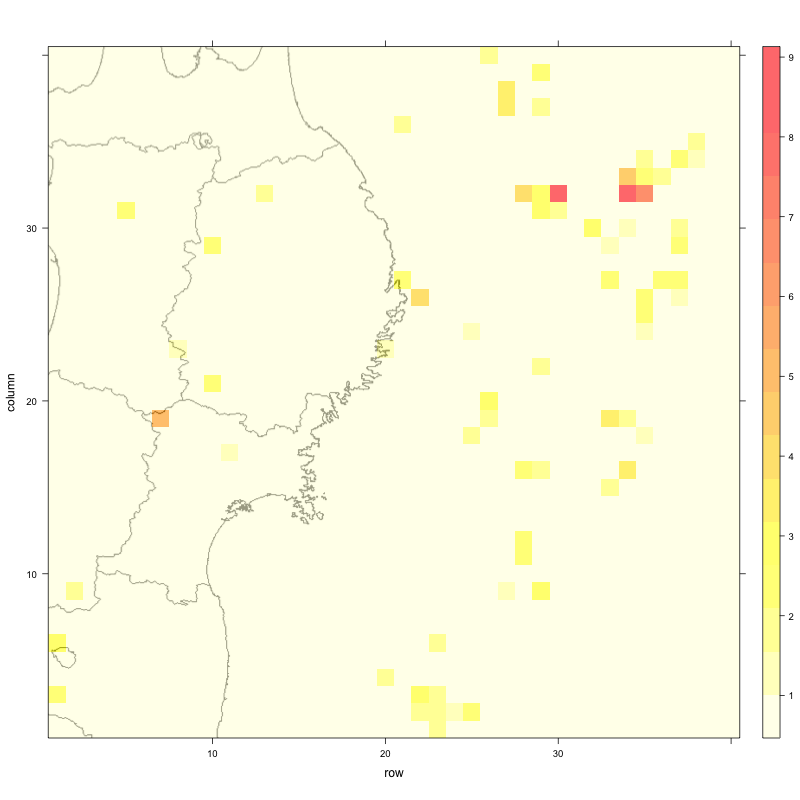
\includegraphics[scale=0.2]{img/gamodel2005eastjapan.png}
%	\label{gamodel2005eastjapan}
%\end{figure}
%
%
%\begin{figure}[H]
%	\centering
%	\begin{minipage}{0.45\textwidth}
%		\centering
%		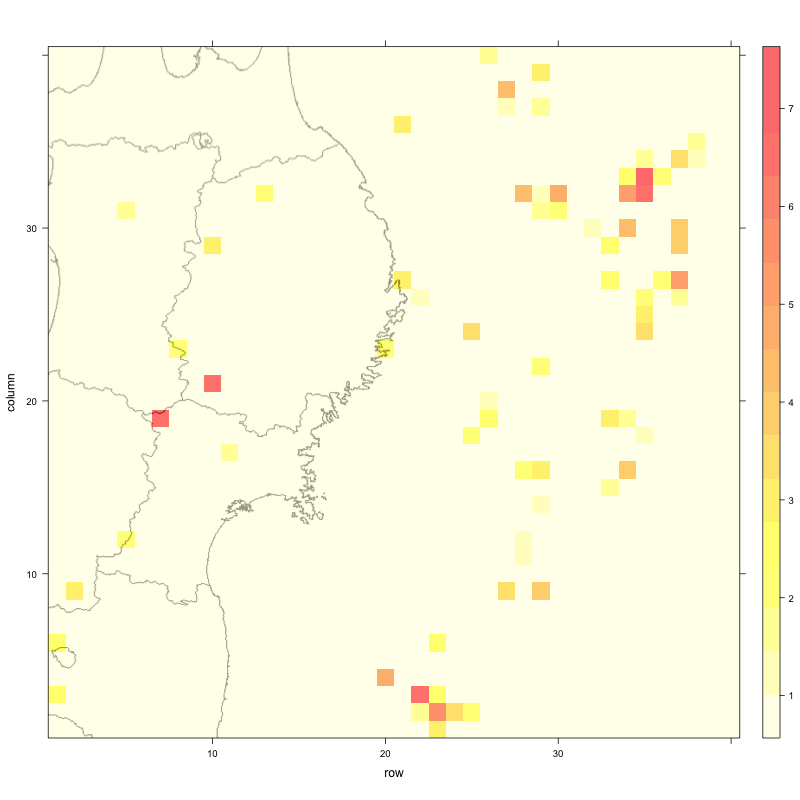
\includegraphics[scale=0.2]{img/reduced2005eastjapan.png}
%		\label{reduced2005eastjapan}
%	\end{minipage}
%	\begin{minipage}{0.45\textwidth}
%		\centering
%		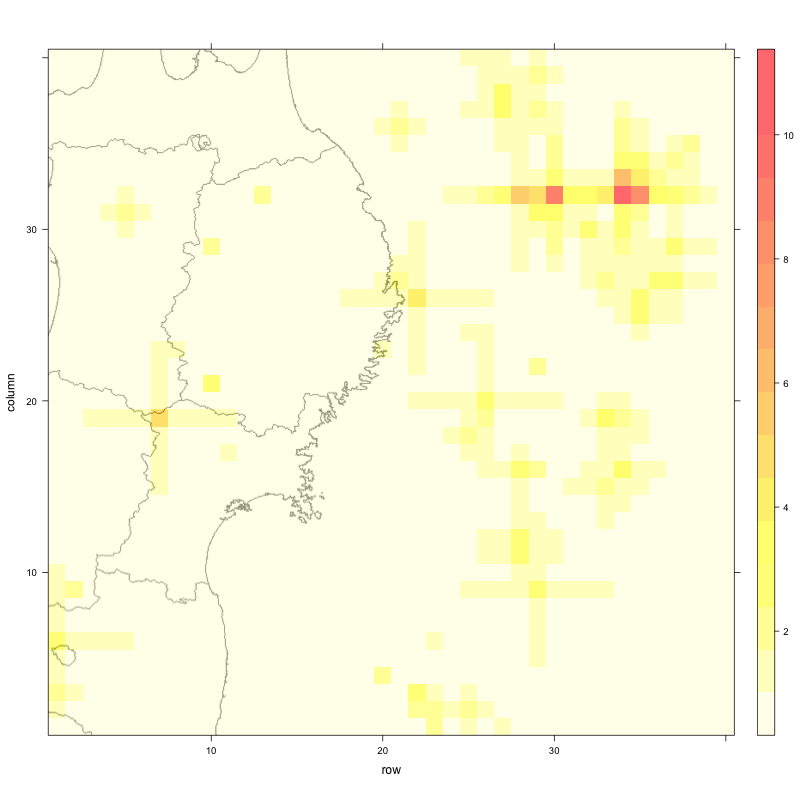
\includegraphics[scale=0.2]{img/hybridgamodel2005eastjapan.png}
%		\label{hybridgamodel2005eastjapan}
%	\end{minipage}
%	\caption{The Figure on the left is the ReducedGAModel model for the year of 2005, East Japan, and the one on the right Emp-GAModel model for the year of 2005, East Japan.}
%\end{figure}
%
%\begin{figure}[H]
%	\begin{minipage}{0.45\textwidth}
%		\centering
%		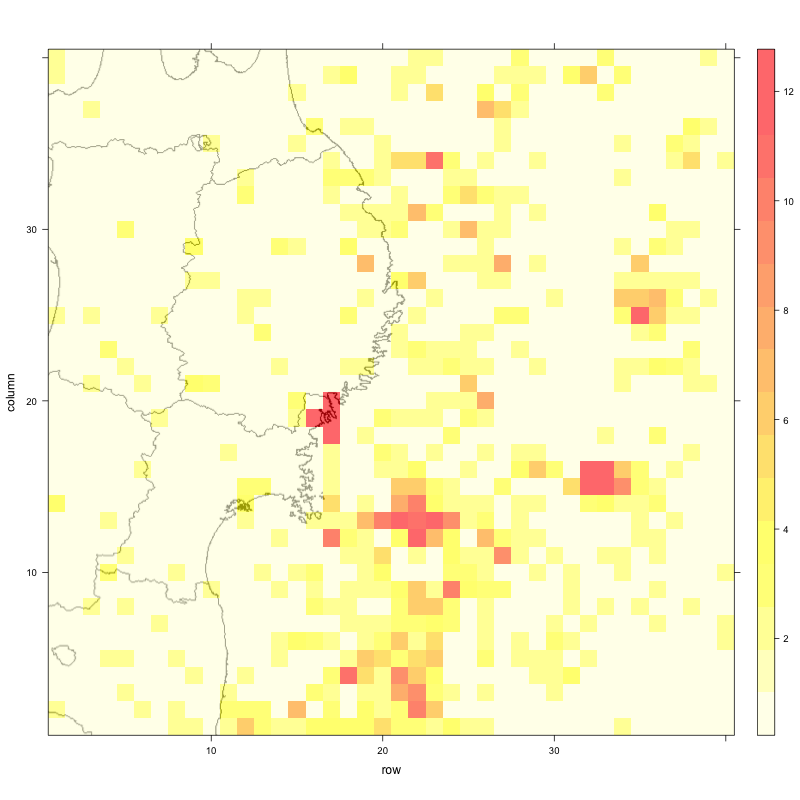
\includegraphics[scale=0.2]{img/real2005eastjapan.png}
%		\caption{Earthquake occurrences in the year of 2005 in East Japan.}
%		\label{real2005eastjapan}
%	\end{minipage}
%	\begin{minipage}{0.45\textwidth}
%		\centering
%		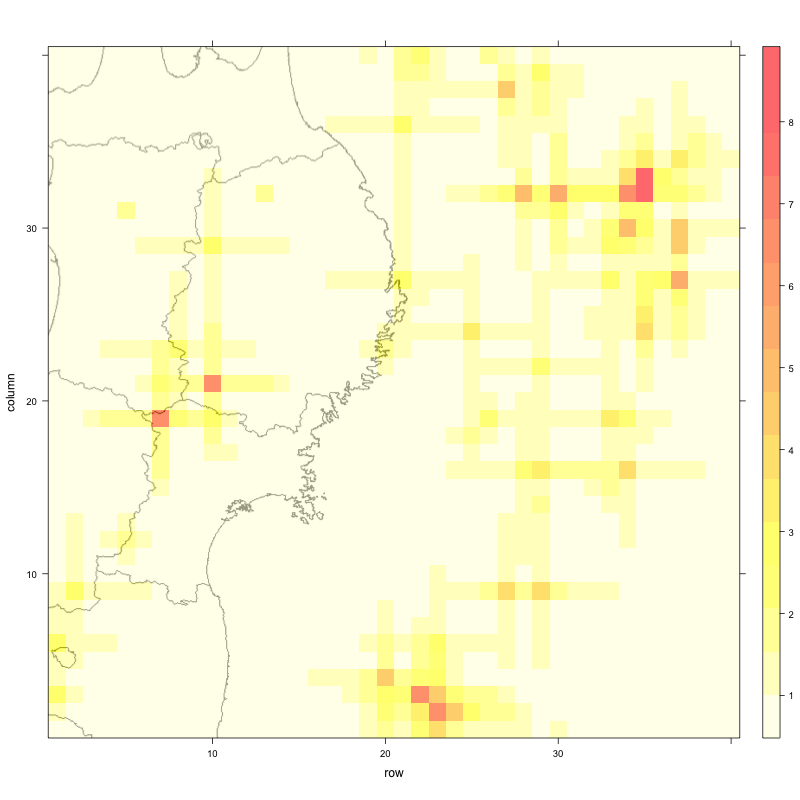
\includegraphics[scale=0.2]{img/hybridreduced2005eastjapan.png}
%		\label{hybridreduced2005eastjapan}
%	\end{minipage}
%	\caption{The Figure on the left is the Emp-ReducedGAModel model for the year of 2005, East Japan, and the one on the right GAModel model for the year of 2005, East Japan, East Japan.}
%\end{figure}




\subsection{Magnitude Experiment}\label{magExp}
The goal is to discover if there is any variation in the methods when considering the magnitude of the earthquakes in the models. We wanted to explore the relation between the magnitude of the earthquakes and how would the models behave on those situations. To achieve that, we used the ANOVA test The confidence interval was set to 95\%.

%For that, we created magnitude intervals, where each interval is named as a slice. A slice is an closed interval of 1.0 degree  starting from 3.0 degrees of magnitude, see~\ref{catalogs}, and ending in 10.0 degrees. For example, $[3.0-4.0]$ or $[7.0-8.0]$ are two different slices. For each model, we selected only the earthquakes that belong to a slice. Then, we calculate the log-likelihood value.
\subsubsection{Magnitude Study}

We compared those split-models against themselves. Based on the results of this test, it is evident that all variables are still significantly different. The results of the ANOVA test are in the Table~\ref{anovatestMag}. For all, as before, we choose the confidence level to be 95\%.

\begin{table*}[!ht]
	\centering
	\begin{tabular}{|l|l|l|l|l|l|}
		\hline
		{Variable} & {Degrees of Freedom} & {Sum Sq}    & {Mean Sq}   & {F Value} & {Pr(\textgreater F)} \\
		\hline
		Model       & 5            	  & 2.360e+09      & 4.720e+08     & 2828     & \textless2e-16     \\
		\hline
		Year        & 3                  & 4.624e+09   & 1.541e+09    & 9234     & \textless2e-16     \\
		\hline
		Magnitude   & 7                  & 3.726e+09   & 5.322e+08    & 3189     & \textless2e-16	\\    
		\hline
	\end{tabular}
	\caption{ANOVA Test Results Values - Magnitude Study.}
	\label{anovatestMag}
\end{table*}

We found statistically significant result and, as before, we applied the Tukey HSD test. It indicated that the interval $[3.0-4.0]$ always performed, in terms of log-likelihood values, worse than all other intervals. this phenomenon also happens in the interval $[4.0-5.0]$, though in this case, the difference is not as big as the last one. The other intervals show no significant difference.

From the results found, we decided to chose only earthquakes with magnitude higher than 4.0 as our threshold value.




%TODO: add future work with Gabriels
%TODO: this section should be a revision of all
